
This chapter give an introduction to literature from the museum field, starting with the ongoing transitional shift to 'a new museology'. The chapter will introduce concepts and terms from exhibition and dissemination practise to extend the vocabulary for talking about museum subjects and roles in the museum. Then we will go into sustainability as a topic representative of a contemporary discourse being addressed in a museum. The chapter will be rounded off with literature on the application of interactivity and interactive installations in "modern museums".

\section{The new museology}

\emph{"The museum world has undergone radical change since the 1970s.  Political and economic pressures have forced its professionals to shift their attention from their collections towards visitors. Whereas in the past the museum tended to be exclusive and elitist, signs of a progressive opening-up and greater accessibility have appeared. A climate of increasing reflexivity within the profession is identified as a ‘new museology’."} \autocite[p. 84]{ross_interpreting_2015}.

The original intention behind the establishment of museums, was that they should remove artefacts from their current context of ownership and use, from their circulation in the world of private property, and insert them into a new environment which would provide them with a different meaning \autocite[p. 6]{vergo_museology_1989}. The essential feature of museums - and what differentiates them from the many extensive private collections which preceded them - was, at first, that the meanings which were attributed to the artefacts were held to be arbitrary; and, second, that the collections should be accessible to at least a portion of the public, who where expected to obtain some form of educational benefit from the experience \autocite[p. 6]{vergo_museology_1989}.

"The museum world is rapidly changing from being collection-centred to being community-centred and for the public. Apart from broadening access to collections through, for example, digitisation initiatives, new ways of involving the public more meaningfully and at various levels have emerged. Experiences inside museums have become more engaging, by extending the experience beyond the physical visit, or by involving the public in various forms of crowd-sourced stewardship of collections." \autocite[abstract]{vermeeren_museum_2018}.

From the book: Museum Experience Design. HCI literature. "four Key Themes of this book: engaging the public, cultivating diverse audiences, availing ourselves of the benefits of digital technology, and leveraging museums’ roles as players in larger economic and cultural ecosystems. "\autocite[abstract]{vermeeren_museum_2018}. "Too often we prioritize our mandate to hold and protect our collections and stop short of making them relevant to today’s audiences, real or potential. Too often we are zoomed way too far in on our objects, and lose sight of what people less invested might know, think, or want from us" \autocite[abstract]{vermeeren_museum_2018}. "In this light, Calvi and Hover’s essay (Chap. 14) is instructive. When we pull our focus back from the individual museum and its obsession with its objects, we find a larger community outside that is largely indifferent to our obsessions, and needs a story, even a superstar, to motivate their interest" \autocite[abstract]{vermeeren_museum_2018}."A struggle emerges between the museum’s role as protector of authentic objects and the “facts” around them and its role as a site of experiences—preferably extraordinary ones, because if not, why bother? "\autocite[abstract]{vermeeren_museum_2018}.

"So, while digital apps take us on mobile adventures and open up trails of wonder for some, the vast majority of our visitors still default to analog first and foremost. The more we can design for blended environments that mix the virtues of analog and digital affordances in mutually reinforcing ways to foster a context for meaningful engagement with museum objects, the better off we’ll be."\autocite[abstract]{vermeeren_museum_2018}.



\section{Exhibition and dissemination practise}

\subsection{Artefact vs artwork}
The ethnographic museum conserves and exhibits artefacts, while the art museum, works of art. It seems obvious what differs the artefact vs the artwork; yet in this section we will learn how the objects they refer to differ regarding what they represent. Both artefacts and artworks is charged with cultural meaning. It tells us about a larger cultural situation, e.g. aesthetic conceptions or world views, conceptions of representations or the social relevance of art. These meanings is only yielded if we are able to “read” it, or is put in some context that illuminates the cultural meaning \autocite[p. 206]{Thi_book}.

The term artefact suggests a man made object charged with cultural meaning which can, if studied carefully, offer us information on the society in which it has been created \autocite[p. 205]{Thi_book}. The difference between the artefact according to the above definition and the common idea of art is that the former takes for granted what the other represses: the possibility of cultural difference. Instead, artworks are viewed as standing for an aesthetic, and is therefore considered metaphors, transferring their specific aesthetic to the one current sufficient to make the work “readable” as art, regardless of what it could tell us about the culture it comes from \autocite[p. 206]{Thi_book}. While the ethnic artefact, in contrast, is first and foremost considered to be a representative of the larger context of the culture it comes from \autocite[p. 206]{Thi_book}. Hence, it is not a metaphor but synecdoche. Synecdoche is the figure of rhetoric where an element, a small part, stands for the whole simply by virtue of its being a part of that whole \autocite[p. 206]{Thi_book}. Thus the artefact is only readable as culture, no matter what aesthetic qualities it may also have.

% need more

\subsection{The curator, concept developer}
The curator are, above all, the institutionally recognised experts of the artworld establishment, whether they operate inside an institution or independently. More than art critics or gallery dealers, they establish the meaning and status of contemporary art through its acquisition, exhibition, and interpretation \autocite[p. 22]{Thi_book}. To a greater extent than other artworld professionals, curators additionally depend on an established infrastructure to support their efforts. This infrastructure includes institutionalised networks, such as those provided by museums, galleries, or alternative spaces; financial sponsors, whether public, private or corporate, and teams of technical or professional experts. Curators are the sanctioned intermediaries of these institutional and professional networks on the one hand, and; artists and audiences on the other. Curatorial function is, this, inherently restricted by the interests of the larger or more powerful groups and constituencies \autocite[p. 22]{Thi_book}.

By selecting, framing and interpreting peripheral art in exhibitions and exhibition catalogues, for instance, art curators can claim to be shaping a more democratic space where specific cultural groups can recognise themselves \autocite[p. 23]{Thi_book}. As the debates of recent years have shown, “identity” is not an “essence” that can be translated into a particular set of conceptual or visual traits. It is, rather a negotiated construct that results from the multiple positions of the subject vis-a-vis the social, cultural and political conditions which contains it. How then, can exhibitions or collections attempt to represent the social, cultural and political complexities of groups without reducing their subjects to essentialist stereotypes? \autocite[p. 23]{Thi_book}.

This situation places the cultural broker at the very core of a contradiction: on one hand, she can be credited for helping to tear down artworld hierarchies, seemingly democratizing the space for cultural action; on the other hand, in a market scenario where “identity” can only be a reductive construct, the framing and packaging of images of the collective self can only result in a highly delusionary enterprise \autocite[p. 23-24]{Thi_book}. The tensions of this contradiction confront art curators with a dilemma. where should they position themselves vis-a-vis the identities of the groups they claim to respect? \autocite[p. 24]{Thi_book}.

\subsection{Dialogical engagement}

"Museums started off as institutions focusing on collecting and preserving objects, open for the public to come and watch. The primary purpose for visitors to come to the museum was to see the original objects. A first notable shift saw the museums move from a collection focus to a visitor focus and from a mission for objects preservation and access provision to a mission of offering meaningful engagements with the collection and rewarding learning experiences for their public. The concept of ‘museum experience’ is the pinnacle of this historical shift, as it implies a focus on the visitor and connections between visitor and objects rather than a focus on collections. In the course of time, new types of museum experiences gradually emerged. The degree of sophistication and immersion increased exponentially when experiences started to be enhanced by the integration of interactive and digital media. In many science and technology museums, for example, visitor engagement and participation are uplifted through the use of new media (e.g. video games, interactive installations and other forms of edutainment) to encourage visitors to engage with the content on exhibit, to experiment with the techniques on show and to appropriate the visiting experience by making it meaningful and memorable. This trend is being adopted also by art museums, where it is by definition more difficult to let visitors experiment with the collections." \autocite[p. 3]{vermeeren_museum_2018}.

\subsection{Museum experience design}



\section{The climate crisis: addressing a contemporary issue}

Traditionally, museums have been a window to the past, "a place where the past lives”. My research aim to provide insight of how museums can play a central role in addressing contemporary issues, like the climate crisis.

The public discussion on the climate crisis is what I refer to as the climate debate. As a museum discourse, the climate debate represents and has some characteristics that open for new ways of thinking on why the museum space is an ideal space for exhibiting the discourse, on new ways of designing for contemporary issues, engaging a broad audience, and using embedded interactivity to design meaningful museum experiences.

\begin{figure}[h]
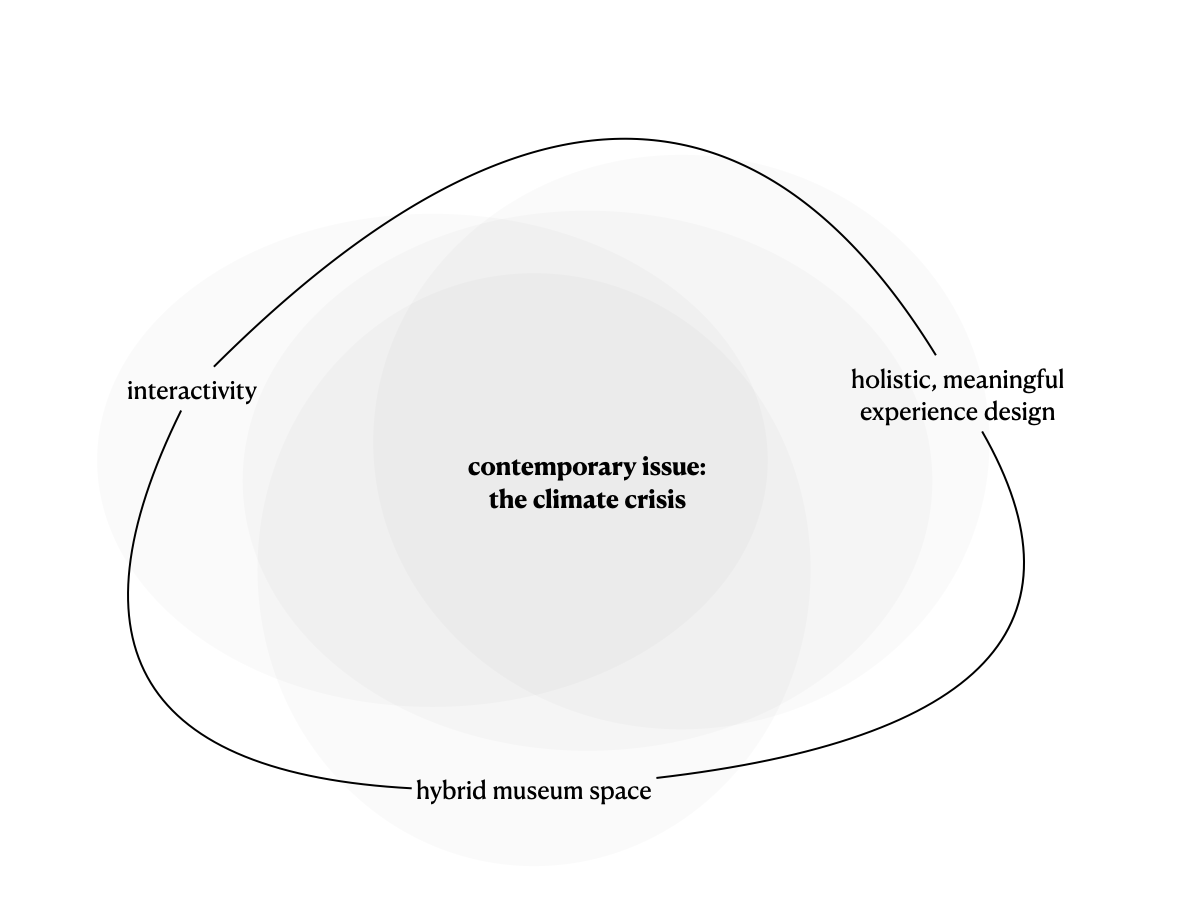
\includegraphics[width=10cm]{pictures/problem_sphere.png}
\caption{My representation of sustainability issues in museums}
\centering
\end{figure}

In a commentary by Richard J. Hebda, it is looked into the Royal British Columbia Museum (RBCM)’s voyage into the issue of climate change as an example of how museums can play a central role in addressing contemporary issues. Traditionally, museums have been a window to the past, "a place where the past lives" \autocite[p. 1]{hebda_article}.  Traditionally, museums trot out historical artifacts, old plant and animal specimens, and host great exhibits on famous people, events and cultures \autocite[p.1]{hebda_article}.
\par
A lot of the issues and societal attitudes that are addressed in the commentary are still relevant today. Traditionally in museums, human and natural history is seen as two solitudes that have been exhibited separately. A key appeal for the RBCM, a typical natural history museum to do a climate change exhibit, was to pursue the opportunity to link and integrate the two solitudes in a compelling and relevant manner \autocite[p. 2]{hebda_article}. They justify that the integration is necessary because the challenge is central in the sustainability debate because the progressive separation of human and natural science is at the core of the problem facing society today \autocite[p.2]{hebda_article}.

In 2007 when the RBCM decided to make the climate change exhibition, the question of climate change was still a controversial issue \autocite[p.2]{hebda_article}. Addressing the increasing evidence and knowledge in terms of climate change and how it affects and is affected by humans, nearly all reputable scientists felt that change was under way and action was needed \autocite[p.2]{hebda_article}. The political and public atmosphere was foggy, as people did not know whom to believe, what information was science-based rather than rhetoric, and where real uncertainty lay \autocite[p.2]{hebda_article}. The RBCM saw a clear opportunity to dispel the fog and to enlighten their audiences \autocite[p.2]{hebda_article}.

To begin with, the museum simply wanted to update the entrance to the natural gallery where climate was briefly explored, but saw the opportunity to create an exhibit where (... this, this and this is adressed). And then write a summary of the case and results of the article.:
- (this was perhaps) a reflection of society’s general lack of recognition of climate’s central role in shaping the world and our lives.
- The museum also struggled with the need to be more socially relevant.

\section{Meaningful interactive experiences}
Hvordar forstår jeg bærekraft, og hvorfor mener jeg det er viktig?
Hvordan snakker andre om det, og hva må jeg få sagt til leseren om bærekraft?
Hvordan “angriper” jeg bærekraft temaet inn i denne oppgaven? 

Hva slags utfordringer er det for museer som tematisk jobber med, /formidler, bærekraft? (Prosess) Hvordan min prosess er farget av det jeg er opptatt av. Rapportering nytt kapittel. Hvordan er prosessen min koblet til teorien?

\begin{figure}[h]
\includegraphics[width=8cm]{pictures/museumintersections.pdf}
\caption{Can the intersection between museal exposition, the museums exposition of arguments and their exposure of cultural artefact provide data or finds on power structures/ tensions/ imbalance in museums? Especially in terms of sustainability?}
\centering
\end{figure}


Mieke Bal is a dutch cultural theorist, video artist and Professor in Literary Theory at the University of Amsterdam, with academic interest and background in humanities, media and culture studies. From her writings on the discourse of the museum, she discusses what differentiates the “new” museology from the “old”, and presents the museum as a discourse and the exhibition as an utterance within that discourse. Bringing this discursive perspective to the museum deprives the museal practise of its innocence, and provides it with the accountability it and its users are entitled to \autocite[p. 214]{Thi_book}. Part of her argument is that politics come straight out of, or more precisely are bound up with, the museal discourse \autocite[p. 214]{Thi_book}, and proposes a threefold direction to museology researchers. First she suggest to systematically analyse the narrative-rhetorical structure of the specific museum, in order to refine the categories and deepen insight into their effects. Secondly she suggest to look at the connection between the museal discourse and the institutions foundation and history, and thirdly she see the need to do self-critical analysis of the museal discourse as a consequence of the nature of discourse.

With my background and scope of thesis it is both irrelevant and I am by no means capable to do a discursive analysis in the way Mieke Bal proposes. I do however find aspects of Bal’s discursive perspective relevant, like her proposal of how one can do a narrative-rhetorical systematic analysis of a specific museum. She provides a set of new terms and vocabulary so that I better can “read”, describe, understand and do research on a specific museum and/ or specific installation. I find this perspective along with the extended vocabulary it provides useful so that I better can identify meaningful relations between user activity at installations/ artefacts and the museum experience.